\section{[Complete] The Screw Axle}

Take a screw, put two nuts on it, and screw them in opposite directions so that they tighten each other. What you have now is a screw axle, where the screw acts as an axle and the two nuts acts like a shaft collar.

Screw axles can be used to attached anything to a metal part securely while still maintaining a degree of freedom. These can be used to make metal whips (steel bars with screw axles), secure encoders loosely, and possibly more. As encoders require a lot of torque to turn if tightened, securing them with screw axles allow unpowered wheels to turn extremely easily.

\begin{figure}[h]
    \centering
    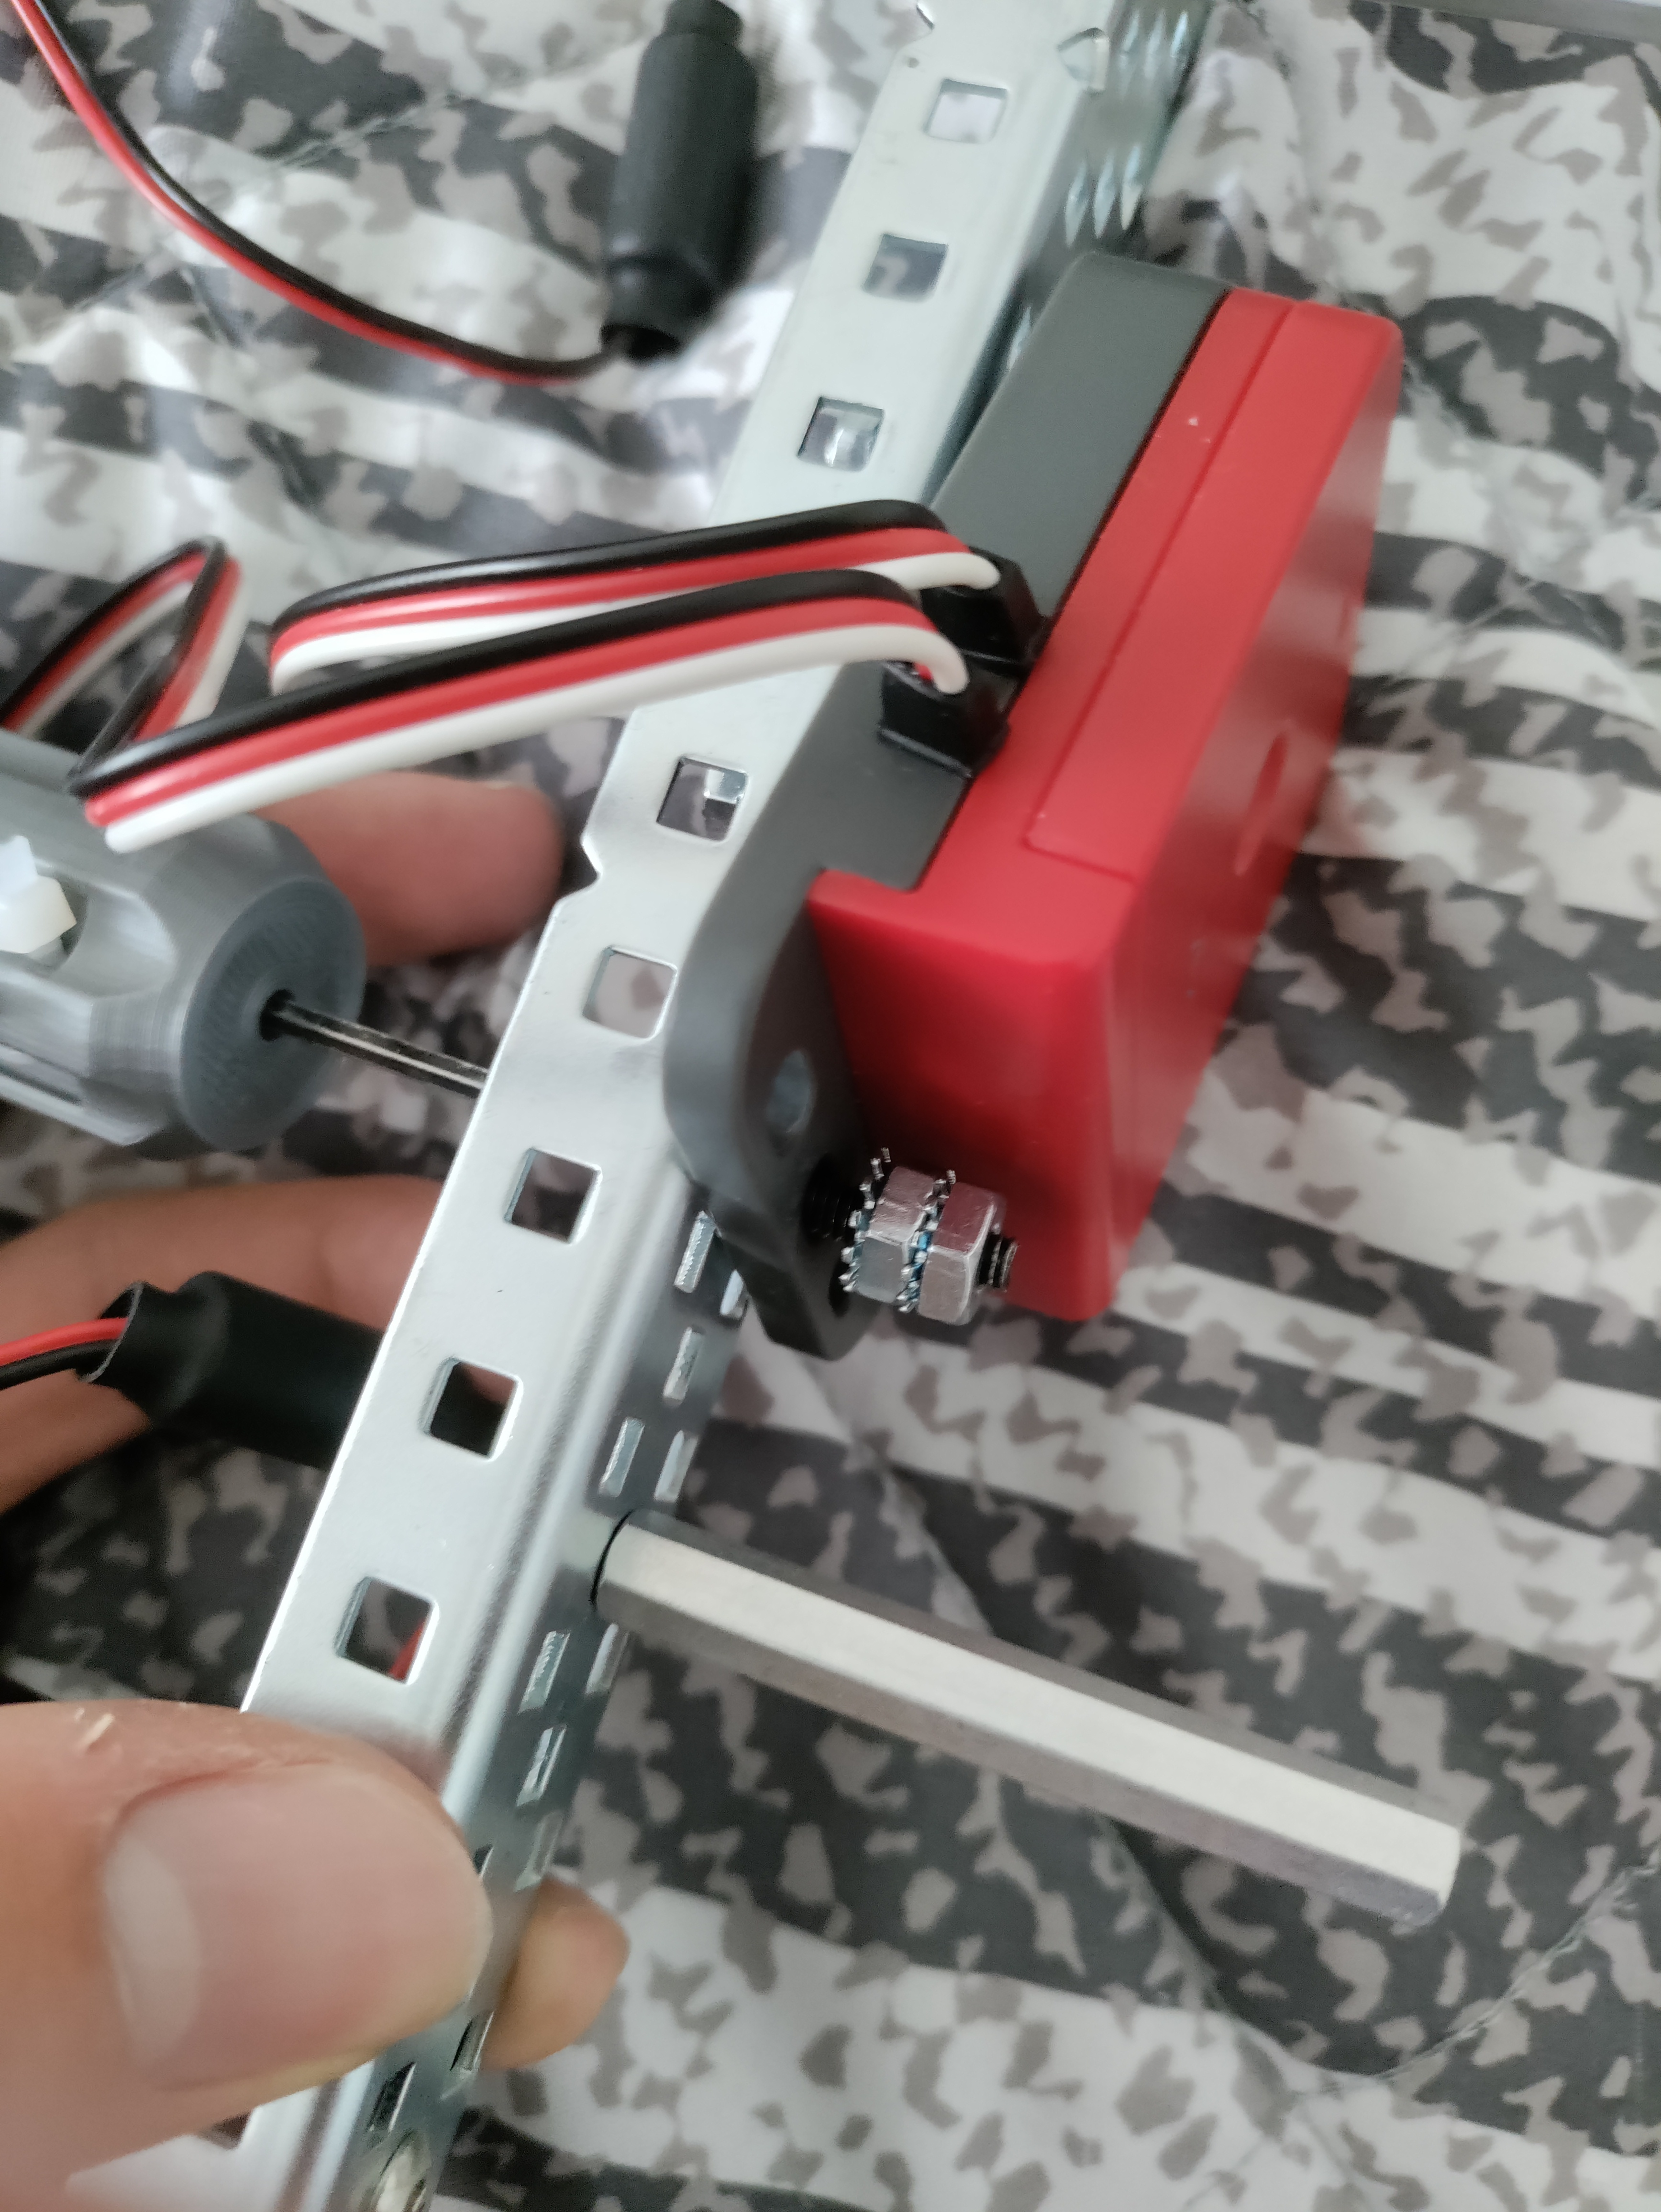
\includegraphics[width=\textwidth,height=9cm,keepaspectratio=true]{ScrewAxle/ScrewAxle}
    \caption{
        A single screw axle being used to attach an encoder to the chassis. The encoder is free to move up and down in the case of axle vibration, and the screw axle prevents it from going anywhere else.
    }
\end{figure}
